\subsubsection{Programmflussdiagramm}
\label{subsubsec:Software_ESP32_Programmflussdiagramm}

\paragraph{Bootloader-Section}\mbox{}\\
In Abbildung \ref{fig:ProgrammflussESP} wird der Programmfluss des Wireless-/Bluetoothmoduls (ESP32) aufgezeigt. Beim Einschalten der Maschine wird das ESP aufgestartet, bevor es in die Init-Section wechselt.

\paragraph{Init-Section}\mbox{}\\
Bei Programmstart werden zuerst die Headerfiles geladen und die Variablen initialisiert, sowie die I/O Schnittstellen und die angeschlossenen Devices. Dabei handelt es sich um das MFRC522-Evalboard (RFID). 

\paragraph{Main-Loop}\mbox{}\\
Das Wireless-/Bluetoothmodul reagiert jeweils auf einkommende Daten. Entweder treffen Daten vom App über Bluetooth ein, vom MFRC522 über SPI oder vom Mikrocontroller via UART. Sobald Daten aus einer dieser Quellen empfangen werden, so reagiert das Programm darauf und löst eine entsprechende Routine aus. 


\begin{figure}[H]
	\centering
	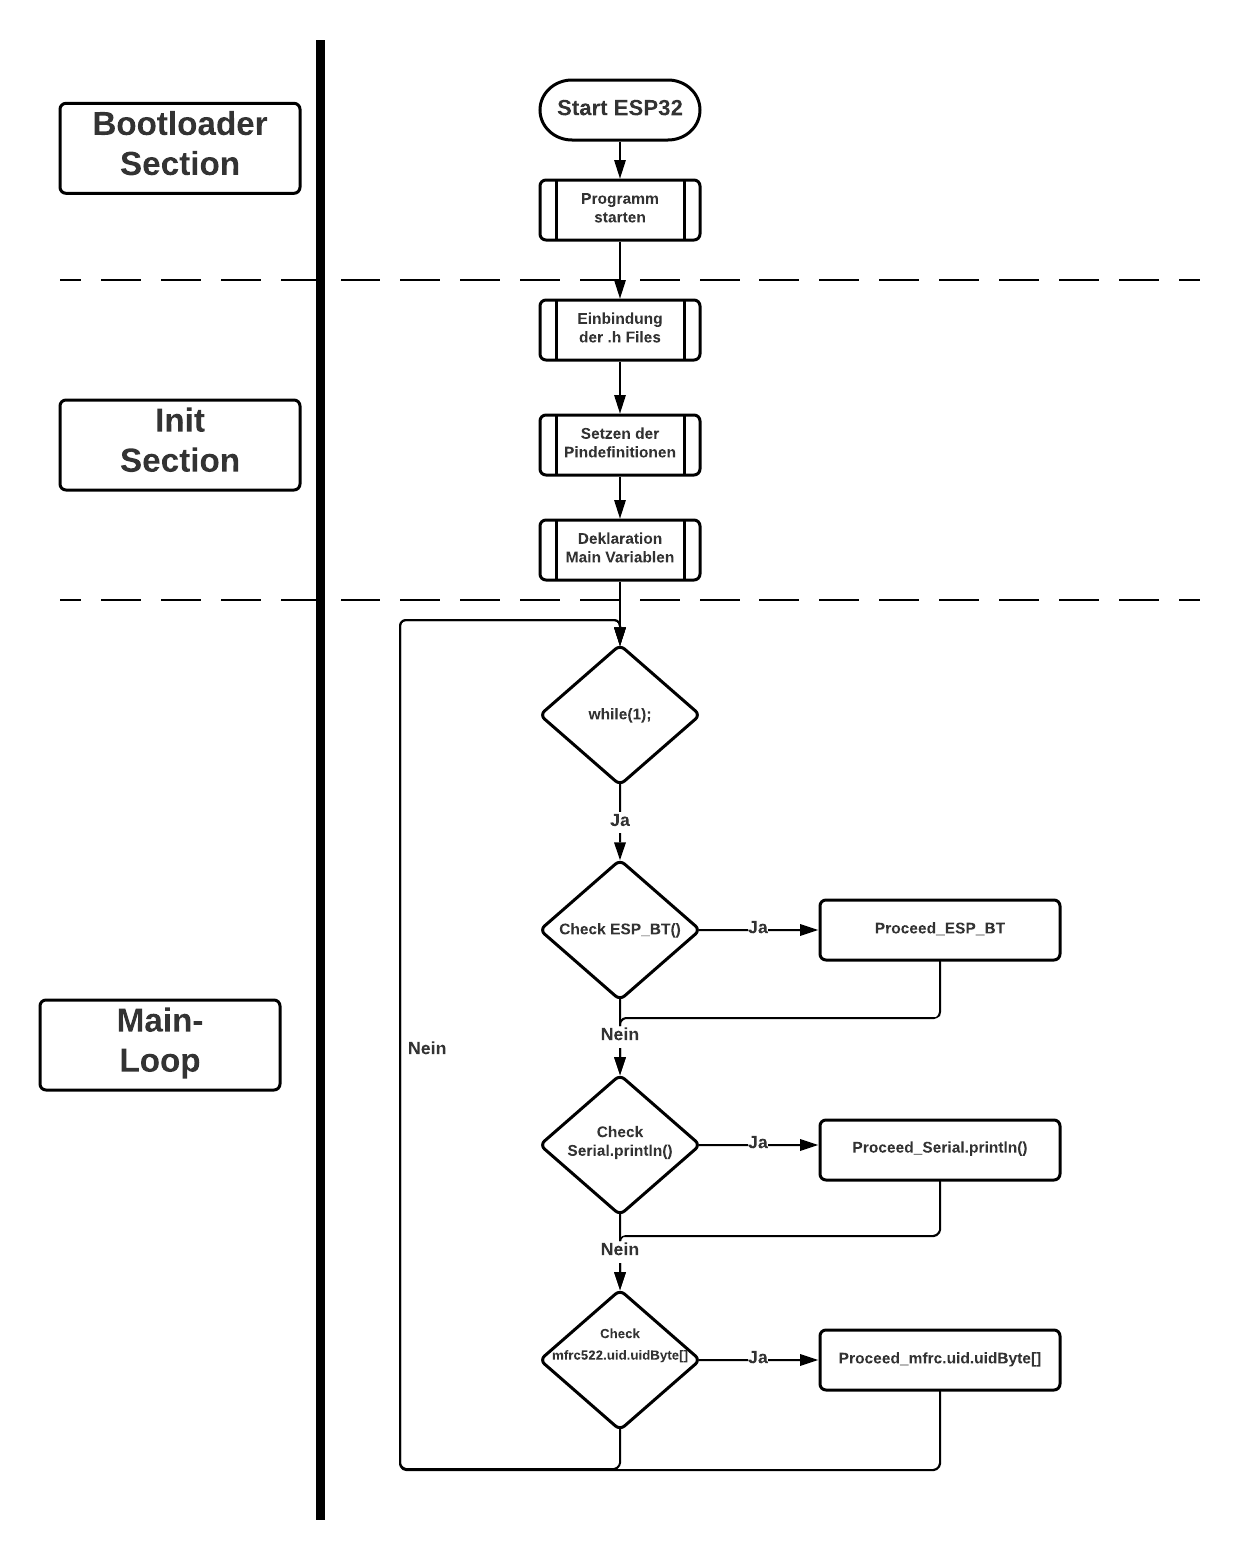
\includegraphics[width=\textwidth]{graphics/ProgrammflussESP}
	\caption{Programmflussdiagramm des ESP32}
	\label{fig:ProgrammflussESP}
\end{figure}
\newpage